\documentclass[11pt, a4paper]{article}

\usepackage{amsmath, amssymb, titling}
\usepackage[margin=2.5cm]{geometry}
\usepackage[colorlinks=true, linkcolor=black, urlcolor=black, citecolor=black]{hyperref}
\usepackage{graphicx}
\usepackage{caption}
\usepackage{subcaption}
\usepackage{float}
\usepackage{multicol}
\usepackage{cancel}
\usepackage{fancyhdr, lastpage}
\usepackage{fourier-orns}
\usepackage{xcolor}
\usepackage{nomencl}
\makenomenclature
\usepackage{etoolbox}
\usepackage{sidecap}
\usepackage{adjustbox}
\usepackage{listings}
\usepackage{matlab-prettifier}
\usepackage[T1]{fontenc}

\sidecaptionvpos{figure}{c}
\setlength{\headheight}{18.2pt}
\setlength{\nomlabelwidth}{1.5cm}

% \renewcommand\maketitlehooka{\null\mbox{}\vfill}
% \renewcommand\maketitlehookd{\vfill\null}

\renewcommand{\headrule}{\vspace{-5pt}\hrulefill\raisebox{-2.1pt}{\quad\leafleft\decoone\leafright\quad}\hrulefill}
\newcommand{\parder}[2]{\frac{\partial {#1}}{\partial {#2}}}
% \renewcommand\nomgroup[1]{%
%   \item[\bfseries
%   \ifstrequal{#1}{F}{Far--Away Properties}{%
%   \ifstrequal{#1}{N}{Dimensionless Numbers}{%
%   \ifstrequal{#1}{M}{Matrices}{%
%   \ifstrequal{#1}{D}{Diagonals}{%
%   \ifstrequal{#1}{V}{Vectors}{%
%   \ifstrequal{#1}{P}{Dimensionless Average Properties}{}}}}}}
% ]}

\title{Numerical Methods in Aeronautical Engineering \\ HW2}
\author{Almog Dobrescu ID 214254252}

% \pagestyle{fancy}
\cfoot{Page \thepage\ of \pageref{LastPage}}

\begin{document}

\thispagestyle{empty}
\begin{figure}[H]
    \centering
    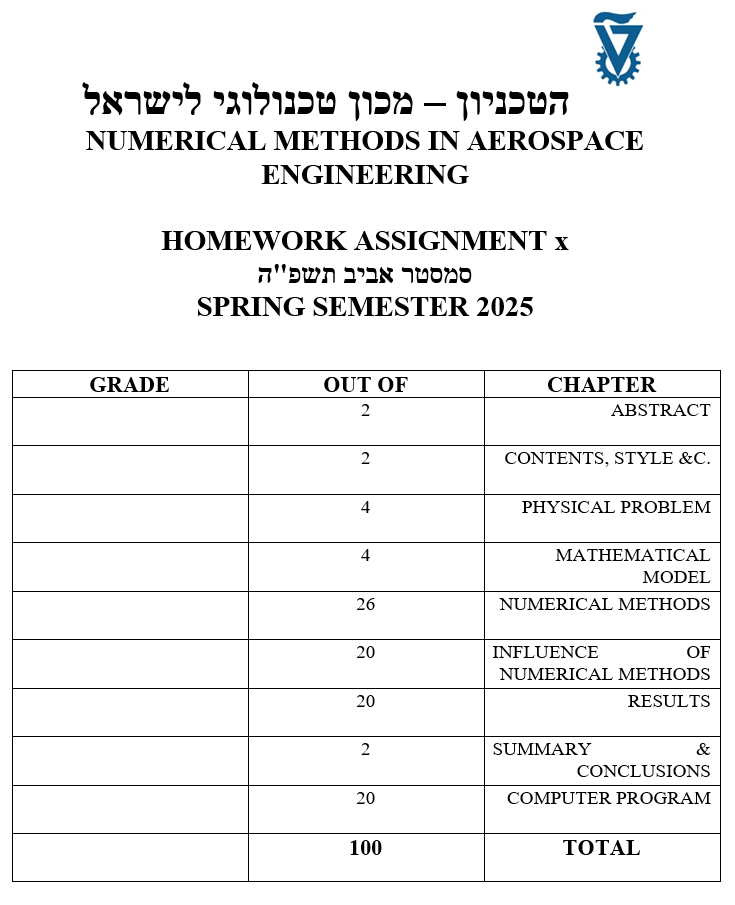
\includegraphics[width=\textwidth]{./../../Cover page for computational assignments 2025.png}
    \label{fig: cover page}
\end{figure}
% \maketitle
\begin{center}
    \Huge
    Almog Dobrescu \qquad ID 214254252 \\ \vspace{0.5cm}
    \today
\end{center}
\newpage

\pagenumbering{roman}
% \setcounter{page}{1}
\begin{abstract}
    Heated tubing has many applications, from water cooling in computers to transporting liquid gas. Research has been conducted to investigate the stress-strain relationships and the material properties of a tube subjected to heating and cooling. A discussion about the optimal parameters was held, and the chosen parameters were used in the results. The results show that the temperature distribution does not depend on the numerical parameter R. The error of the temperature distribution between two convergence criteria decreases exponentially with the decrease of $\varepsilon$.
\end{abstract}

\tableofcontents
\vfil
\listoffigures
\vfil
\lstlistoflistings
\newpage

\printnomenclature
\newpage

\pagestyle{fancy}
\pagenumbering{arabic}
\setcounter{page}{1}

\section{The Physical Problem}
Heated tubing has many applications, from water cooling in computers to transporting liquid gas. Research has been conducted to investigate the stress-strain relationships and the material properties of a tube subjected to heating and cooling.

\section{The Mathematical Model}
The following heat equation was in use:
\begin{equation}
    \begin{matrix}
        \displaystyle\frac{1}{4K}\parder{T}{t}=\parder{^2T}{r^2}+\frac{1}{r}\parder{T}{r} & , & \displaystyle\frac{1}{2}\le r\le1 & , & 0<t
    \end{matrix}
    \nomenclature{$T$}{temperature}
    \nomenclature{$K$}{diffusivity coefficient}
    \nomenclature{$r$}{radiaul coordinate}
    \nomenclature{$t$}{time coordinate}
\end{equation}
The boundary and initial conditions of the problem:
\begin{equation}
    \begin{array}{lcl}
        \displaystyle T_{\left(0.5,t\right)} & = & t \\
        \displaystyle T_{\left(1.0,t\right)} & = & 100+40t \\
        \displaystyle T_{\left(r,0\right)} & = & \displaystyle200\left(r-\frac{1}{2}\right) \\
        \displaystyle K & = & 0.1 \\
    \end{array}
\end{equation}
The strain \emph{I} is given by the equation:
\begin{equation}
    I=\int_{0.5}^{1}{\alpha T_{\left(r,t\right)}rdr}
\end{equation}
\begin{itemize}
    \item $\alpha=10.7$
\end{itemize}

\section{The Numerical Methods}
\subsection{Finite Differencing}
The Heat equation can be rewritten as:
\begin{equation}
    \displaystyle \parder{T}{t}=4K\left(\parder{^2T}{r^2}+\frac{1}{r}\parder{T}{r}\right)
\end{equation}
By using central differencing for the spatial derivatives and forward differencing for the time derivative we get the explicit scheme:
\begin{equation*}
    \displaystyle \frac{T_{i,j+1}-T_{i,j}}{\Delta t}+\emph{O}\left(\Delta t\right)=4K\left(\frac{T_{i-1,j}-2T_{i,j}+T_{i+1,j}}{\Delta r^2}+\emph{O}\left(\Delta r^2\right)+\frac{1}{r}\frac{T_{i+1,j}-T_{i-1,j}}{2\Delta r}+\emph{O}\left(\Delta r^2\right)\right)
\end{equation*}
\begin{equation*}
    \Downarrow
\end{equation*}
\begin{equation}
    \begin{array}{c}
        \displaystyle T_{i,j+1}=T_{i,j}+4K\Delta t\left(\frac{T_{i-1,j}-2T_{i,j}+T_{i+1,j}}{\Delta r^2}+\frac{1}{r}\frac{T_{i+1,j}-T_{i-1,j}}{2\Delta r}\right)+\emph{O}\left(\Delta t, \Delta r^2\right) \\\\
        \displaystyle T_{i,j+1}=T_{i,j}+4KR\left(T_{i-1,j}-2T_{i,j}+T_{i+1,j}+\frac{\Delta r}{2r}\left(T_{i+1,j}-T_{i-1,j}\right)\right)+\emph{O}\left(\Delta t, \Delta r^2\right)
    \end{array}
    \nomenclature{$i$}{index in coordinate r}
    \nomenclature{$j$}{index in time}
    \nomenclature{$\Delta r$}{difference between two points in space}
    \nomenclature{$\Delta t$}{difference between two points in time}
\end{equation}
\begin{multicols}{2}
    \begin{itemize}
        \item $i=1,2,\cdots,N$
        \item $j=1,2,\cdots,J$
        \item $R=\displaystyle\frac{\Delta t}{\Delta r^2}$
        \item $T_{\left(i=0,j\right)}=j\cdot\Delta t$
        \item $T_{\left(i=N+1,j\right)}=100+40\cdot j\cdot\Delta t$
        \item $T_{\left(i,j=0\right)}=200\left(r-\displaystyle\frac{1}{2}\right),\ 0\le r\le N+1$
        \nomenclature{$N$}{number of cell}
        \nomenclature{$J$}{final time coordinate}
    \end{itemize}
\end{multicols}
\noindent $\Delta r$ was calculated as follows:
\begin{equation}
    \Delta r=\frac{r_\text{max}-r_\text{min}}{N+1}
\end{equation}
The step size in time $\Delta t$ was chosen somewhat arbitrary, only to maintain stability.\\

\noindent The system of equation will be solved by Jacobi method for every \emph{j}. This method adds an iterative index \emph{n}:
\begin{equation}
    \displaystyle T_{i,j+1}^{n+1}=T_{i,j}^n+4KR\left(T_{i-1,j}^n-2T_{i,j}^n+T_{i+1,j}^n+\frac{\Delta r}{2r}\left(T_{i+1,j}^n-T_{i-1,j}^n\right)\right)
\end{equation}

\subsection{Convergence Criteria}
In order determined if the iterative method for solving the system of equation has converged, we will check if the temperature vector at a specific time has changed from step \emph{n} to step \emph{n+1} in the following way:
\begin{equation}
    \left|T_{i,j}^{n+1}-T_{i,j}^n\right|<\varepsilon
    \nomenclature{$\varepsilon$}{convergence criteria}
\end{equation}

\subsection{Integral Calculation}
The integral to calculate the strain \emph{I} will be calculated using trapezoid integration:
\begin{equation}
    I=\alpha\frac{h}{2}\sum_{i=0}^{N}{T_{\left(i+1\right)}+T_{\left(i\right)}}
\end{equation}

\section{Influence of The Numerical Methods}
NOTE - the temperature will be presented in logarithmic scale.
\subsection{Influence of Number of Elements N}
\begin{figure}[H]
    \centering
    \begin{subfigure}[c]{0.49\textwidth}
        \centering
        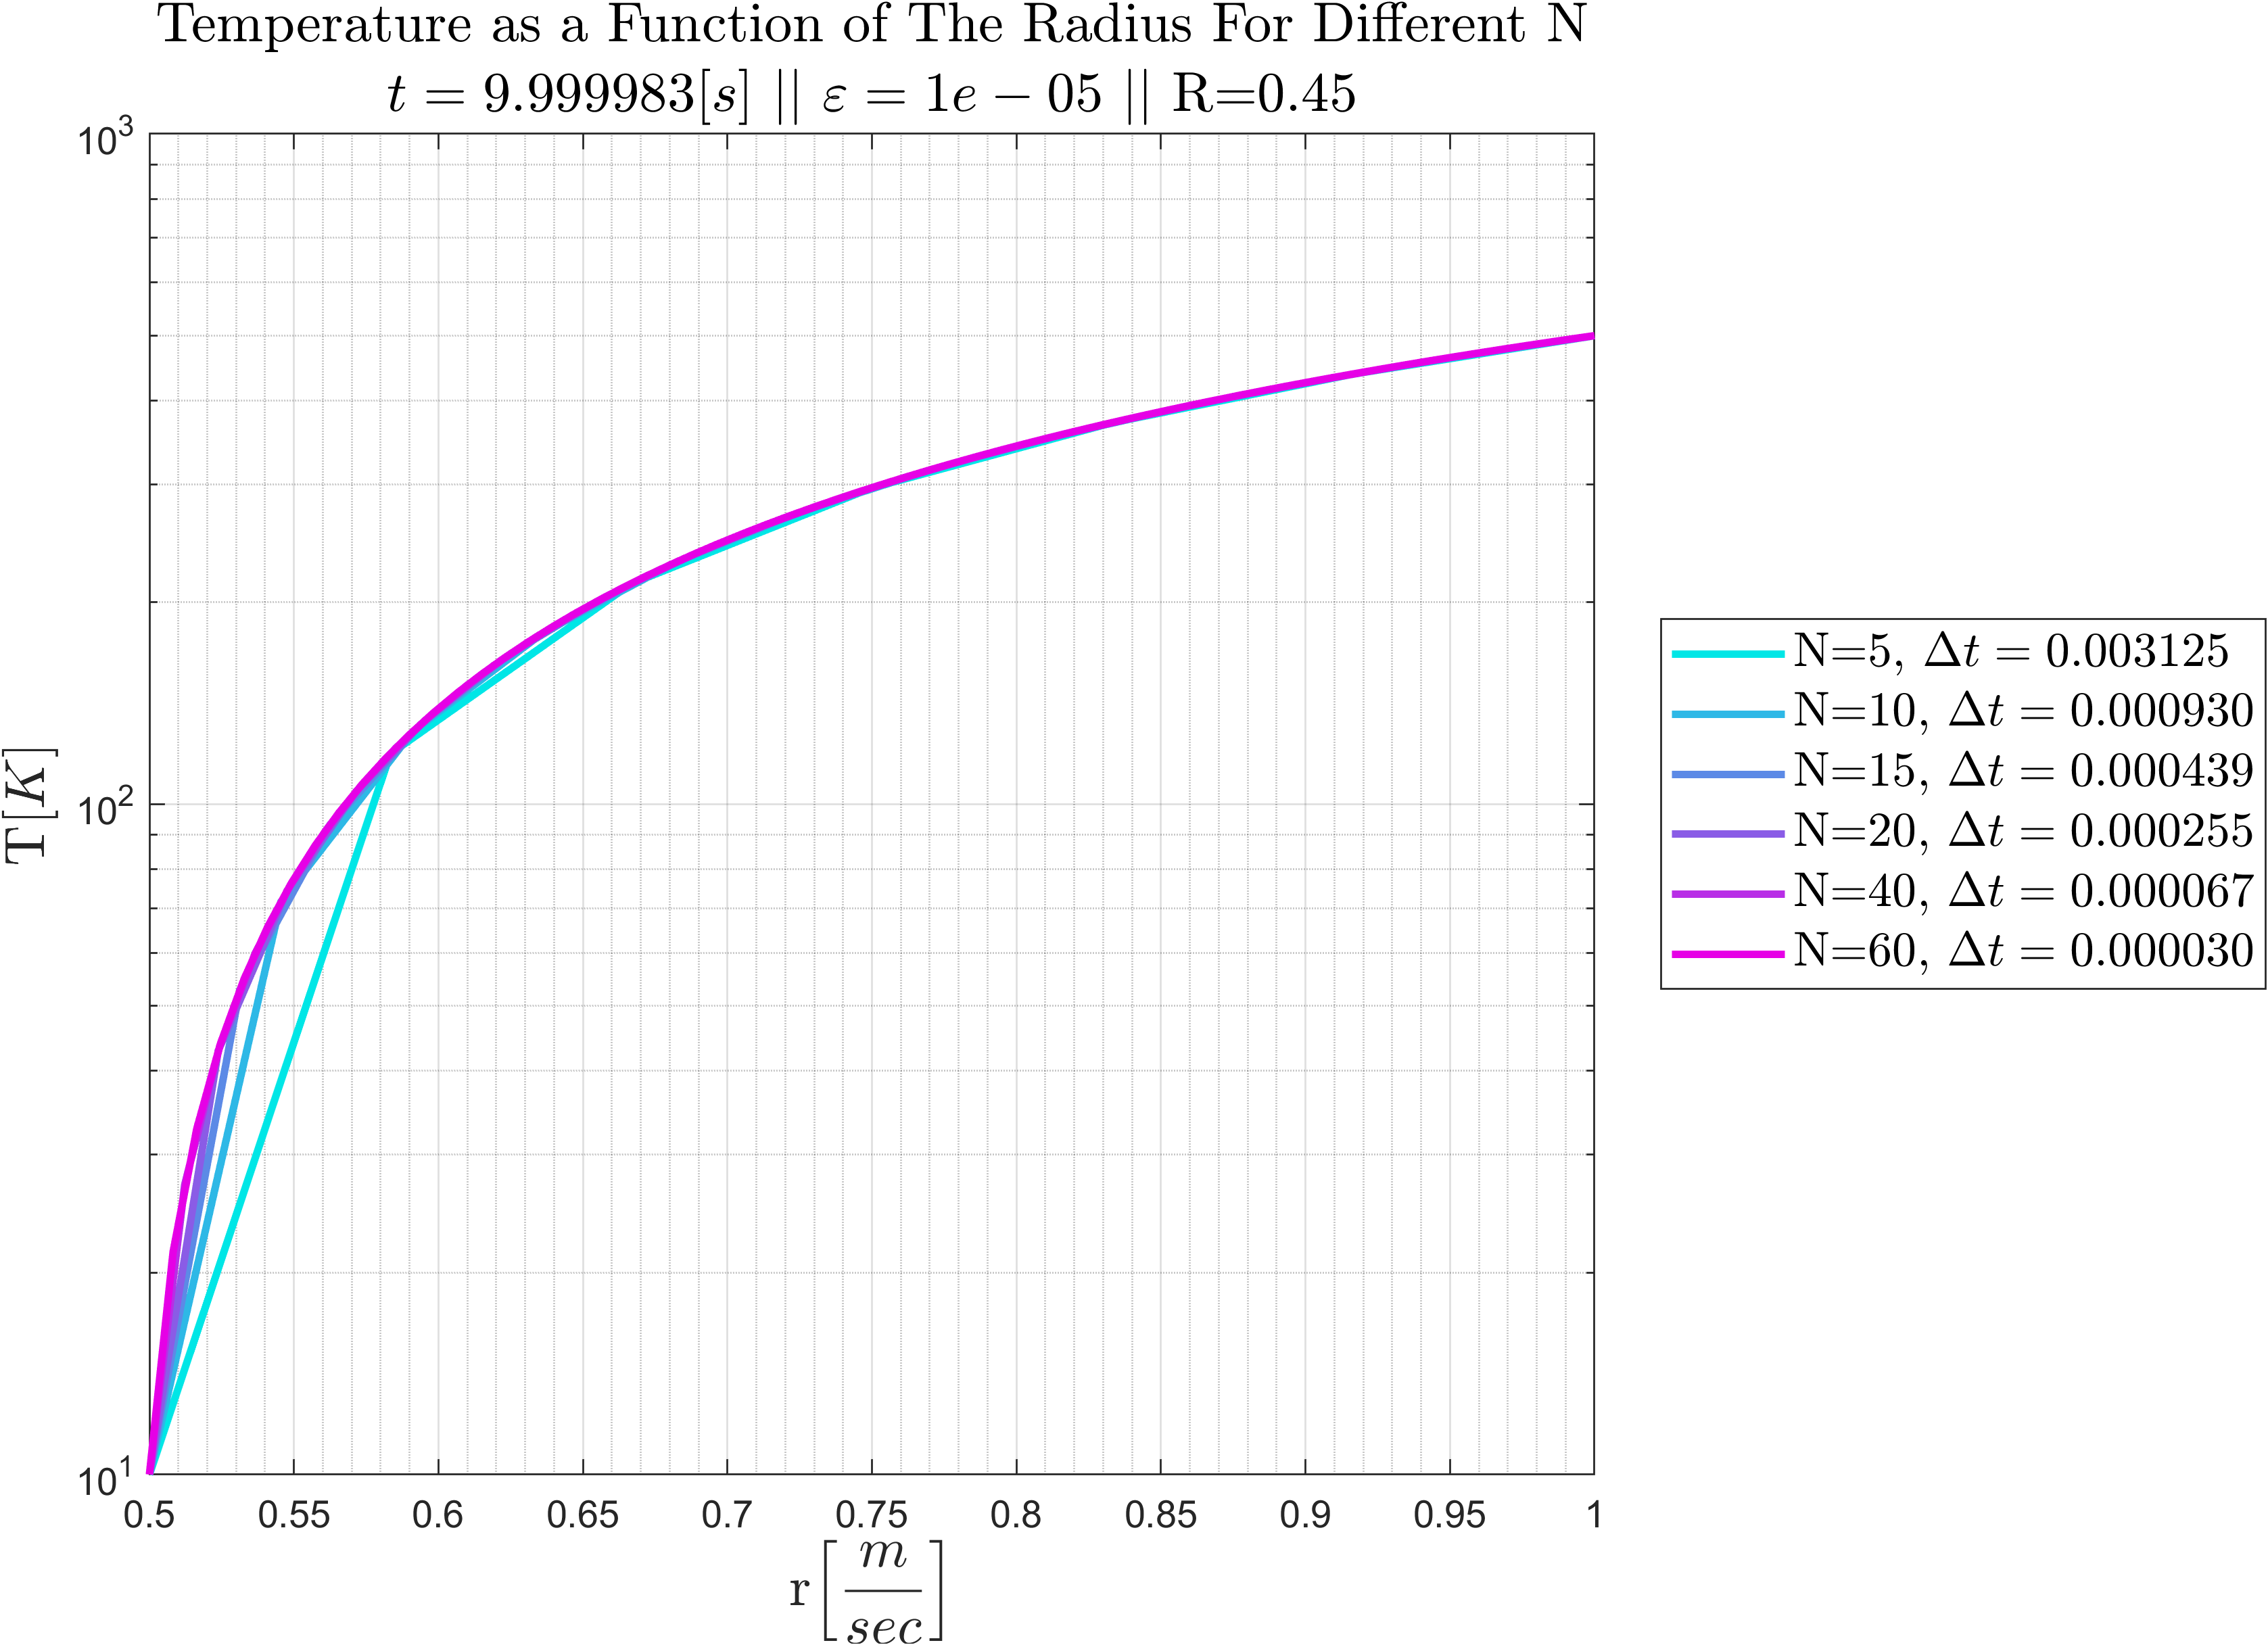
\includegraphics[width=\textwidth]{images/Influenc of N.png}
        \caption{Temperature as a Function of r for different N}
        \label{fig: T vs r for diff N}
    \end{subfigure}
    \hfill
    \begin{subfigure}[c]{0.49\textwidth}
        \centering
        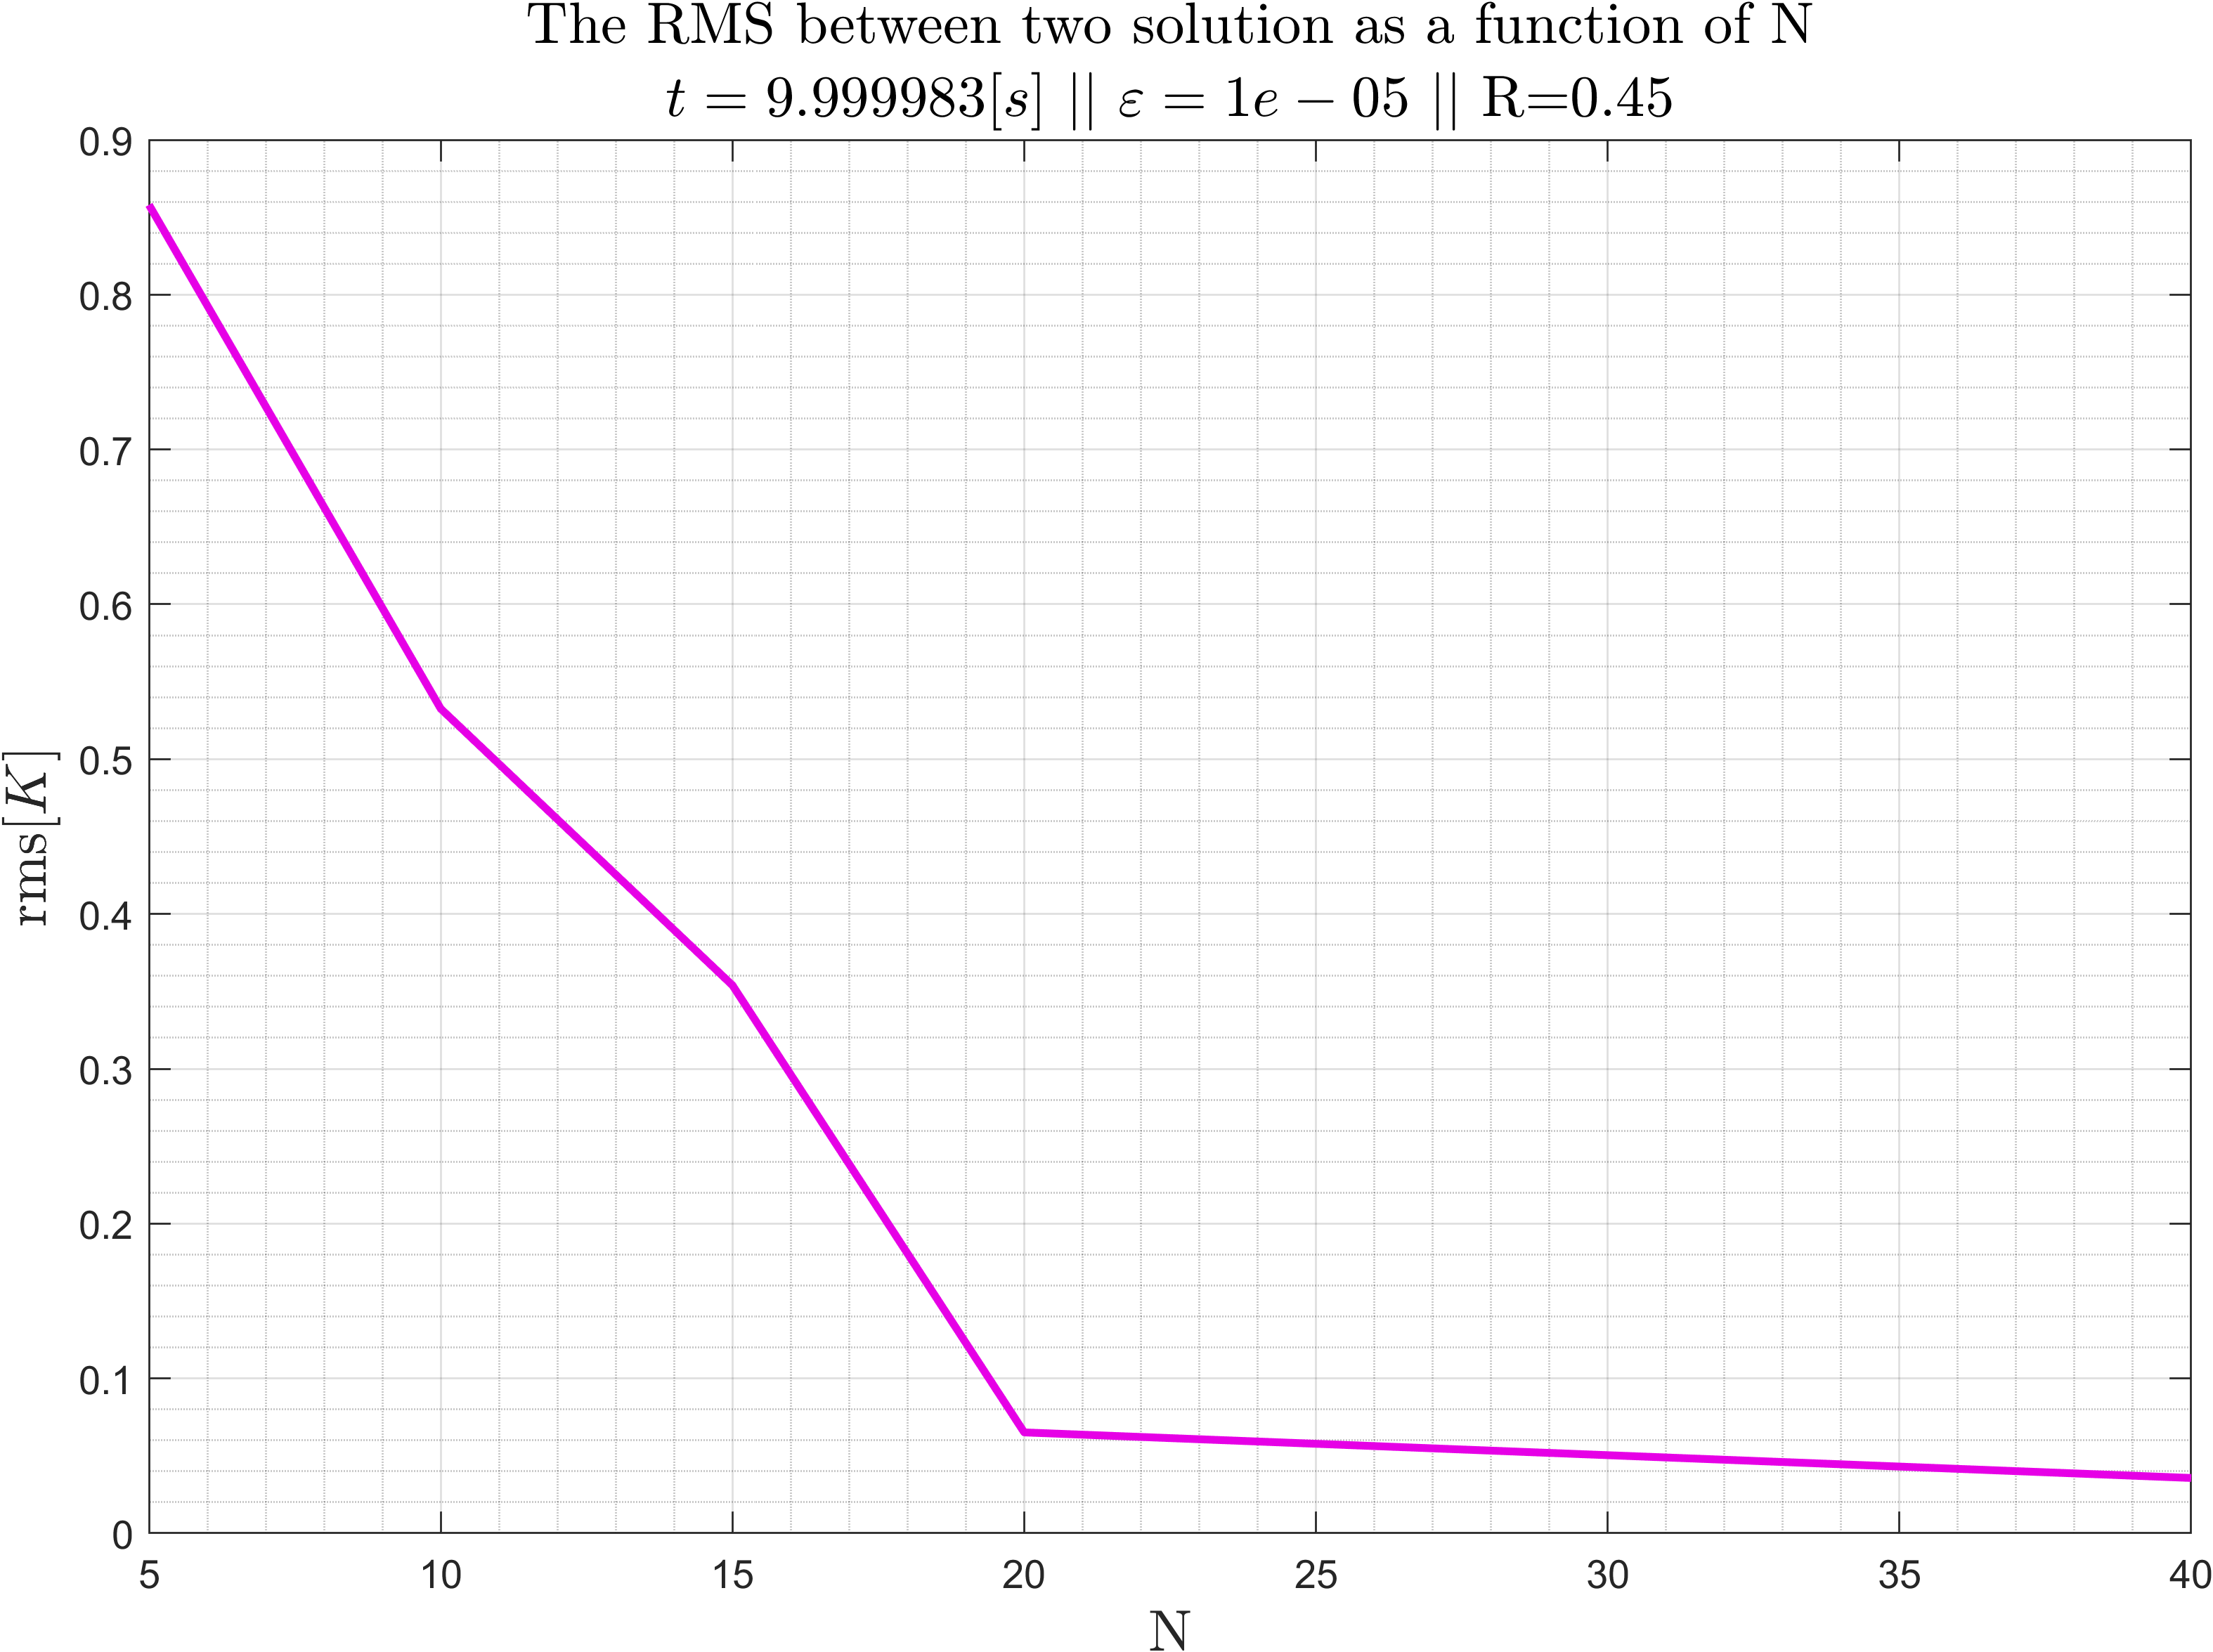
\includegraphics[width=\textwidth]{images/Influenc of N - error.png}
        \caption{RMS as a function of N}
        \label{fig: RMS vs N}
    \end{subfigure}
    \caption{Influence of the number of elements N}
    \label{fig: Influence of N}
\end{figure}
In Fig.\ref{fig: Influence of N} we can see that for N bigger than 20, the solution does not really change. We can conclude that $N=20$ is a sufficient number of elements.

\subsection{Influence of Convergence Criteria $\varepsilon$}
\begin{figure}[H]
    \centering
    \begin{subfigure}[c]{0.49\textwidth}
        \centering
        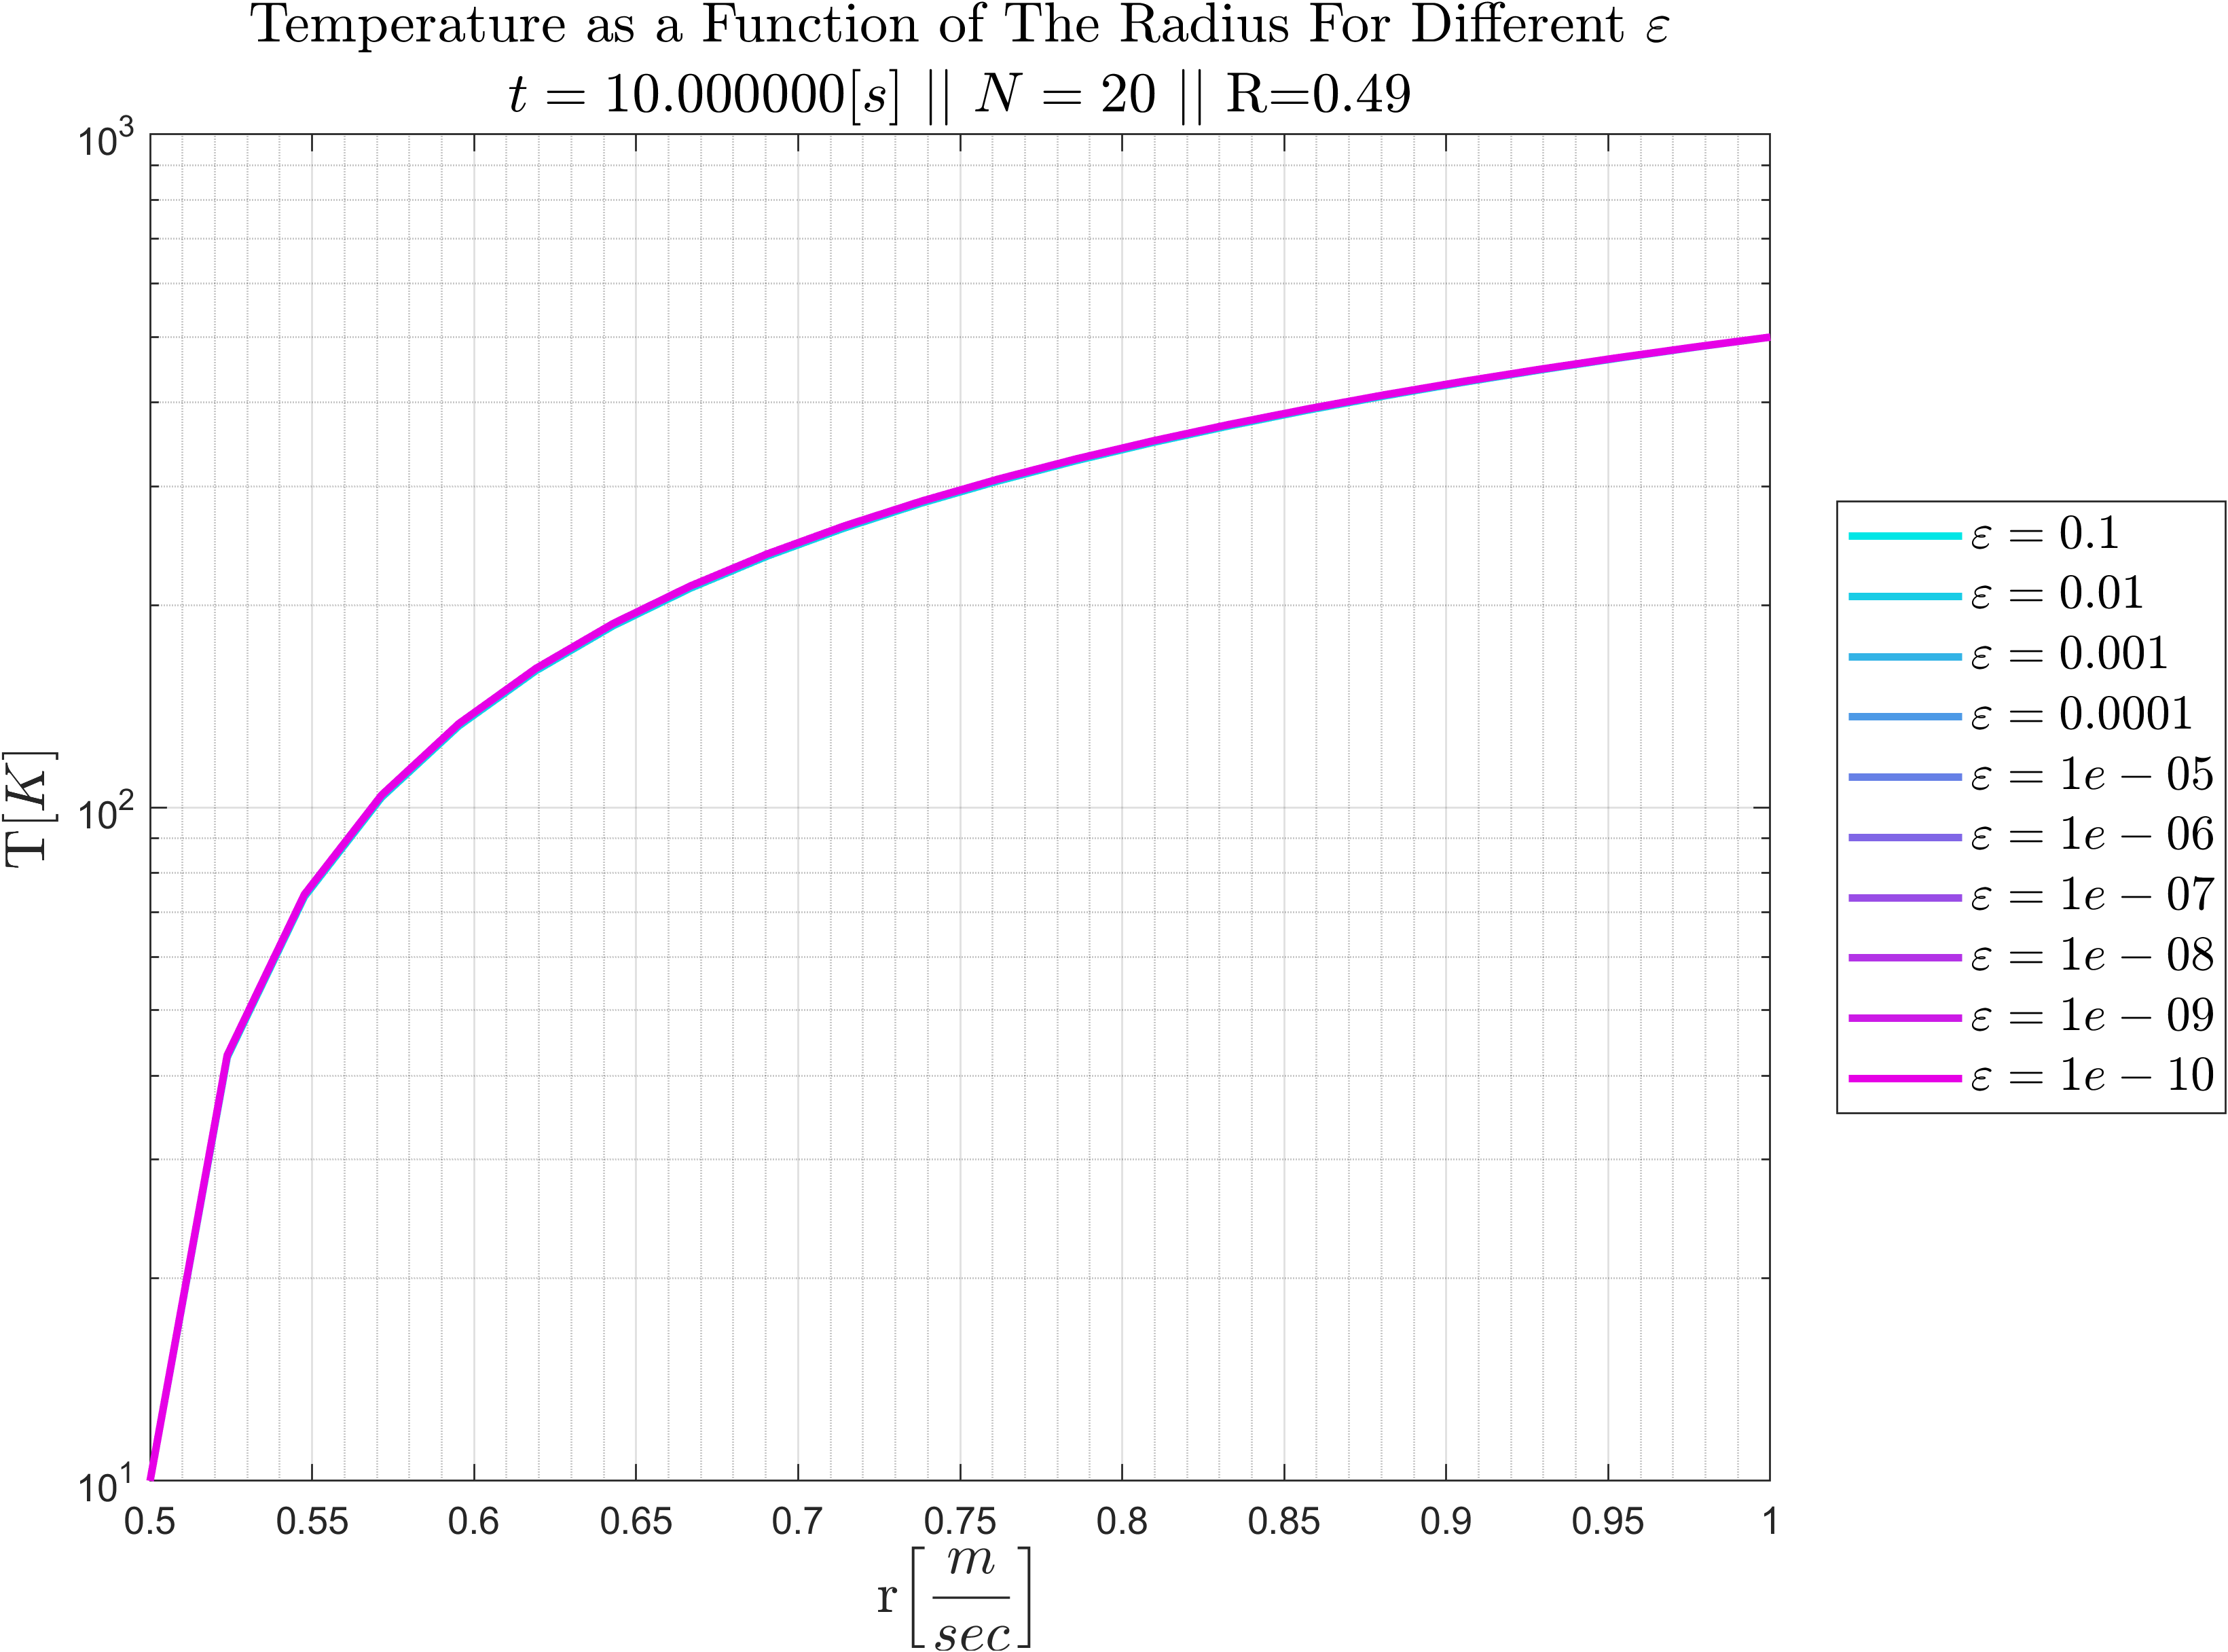
\includegraphics[width=\textwidth]{images/Influenc of epsilon.png}
        \caption{Temperature as a Function of r for different $\varepsilon$}
        \label{fig: T vs r for diff epsilon}
    \end{subfigure}
    \hfill
    \begin{subfigure}[c]{0.49\textwidth}
        \centering
        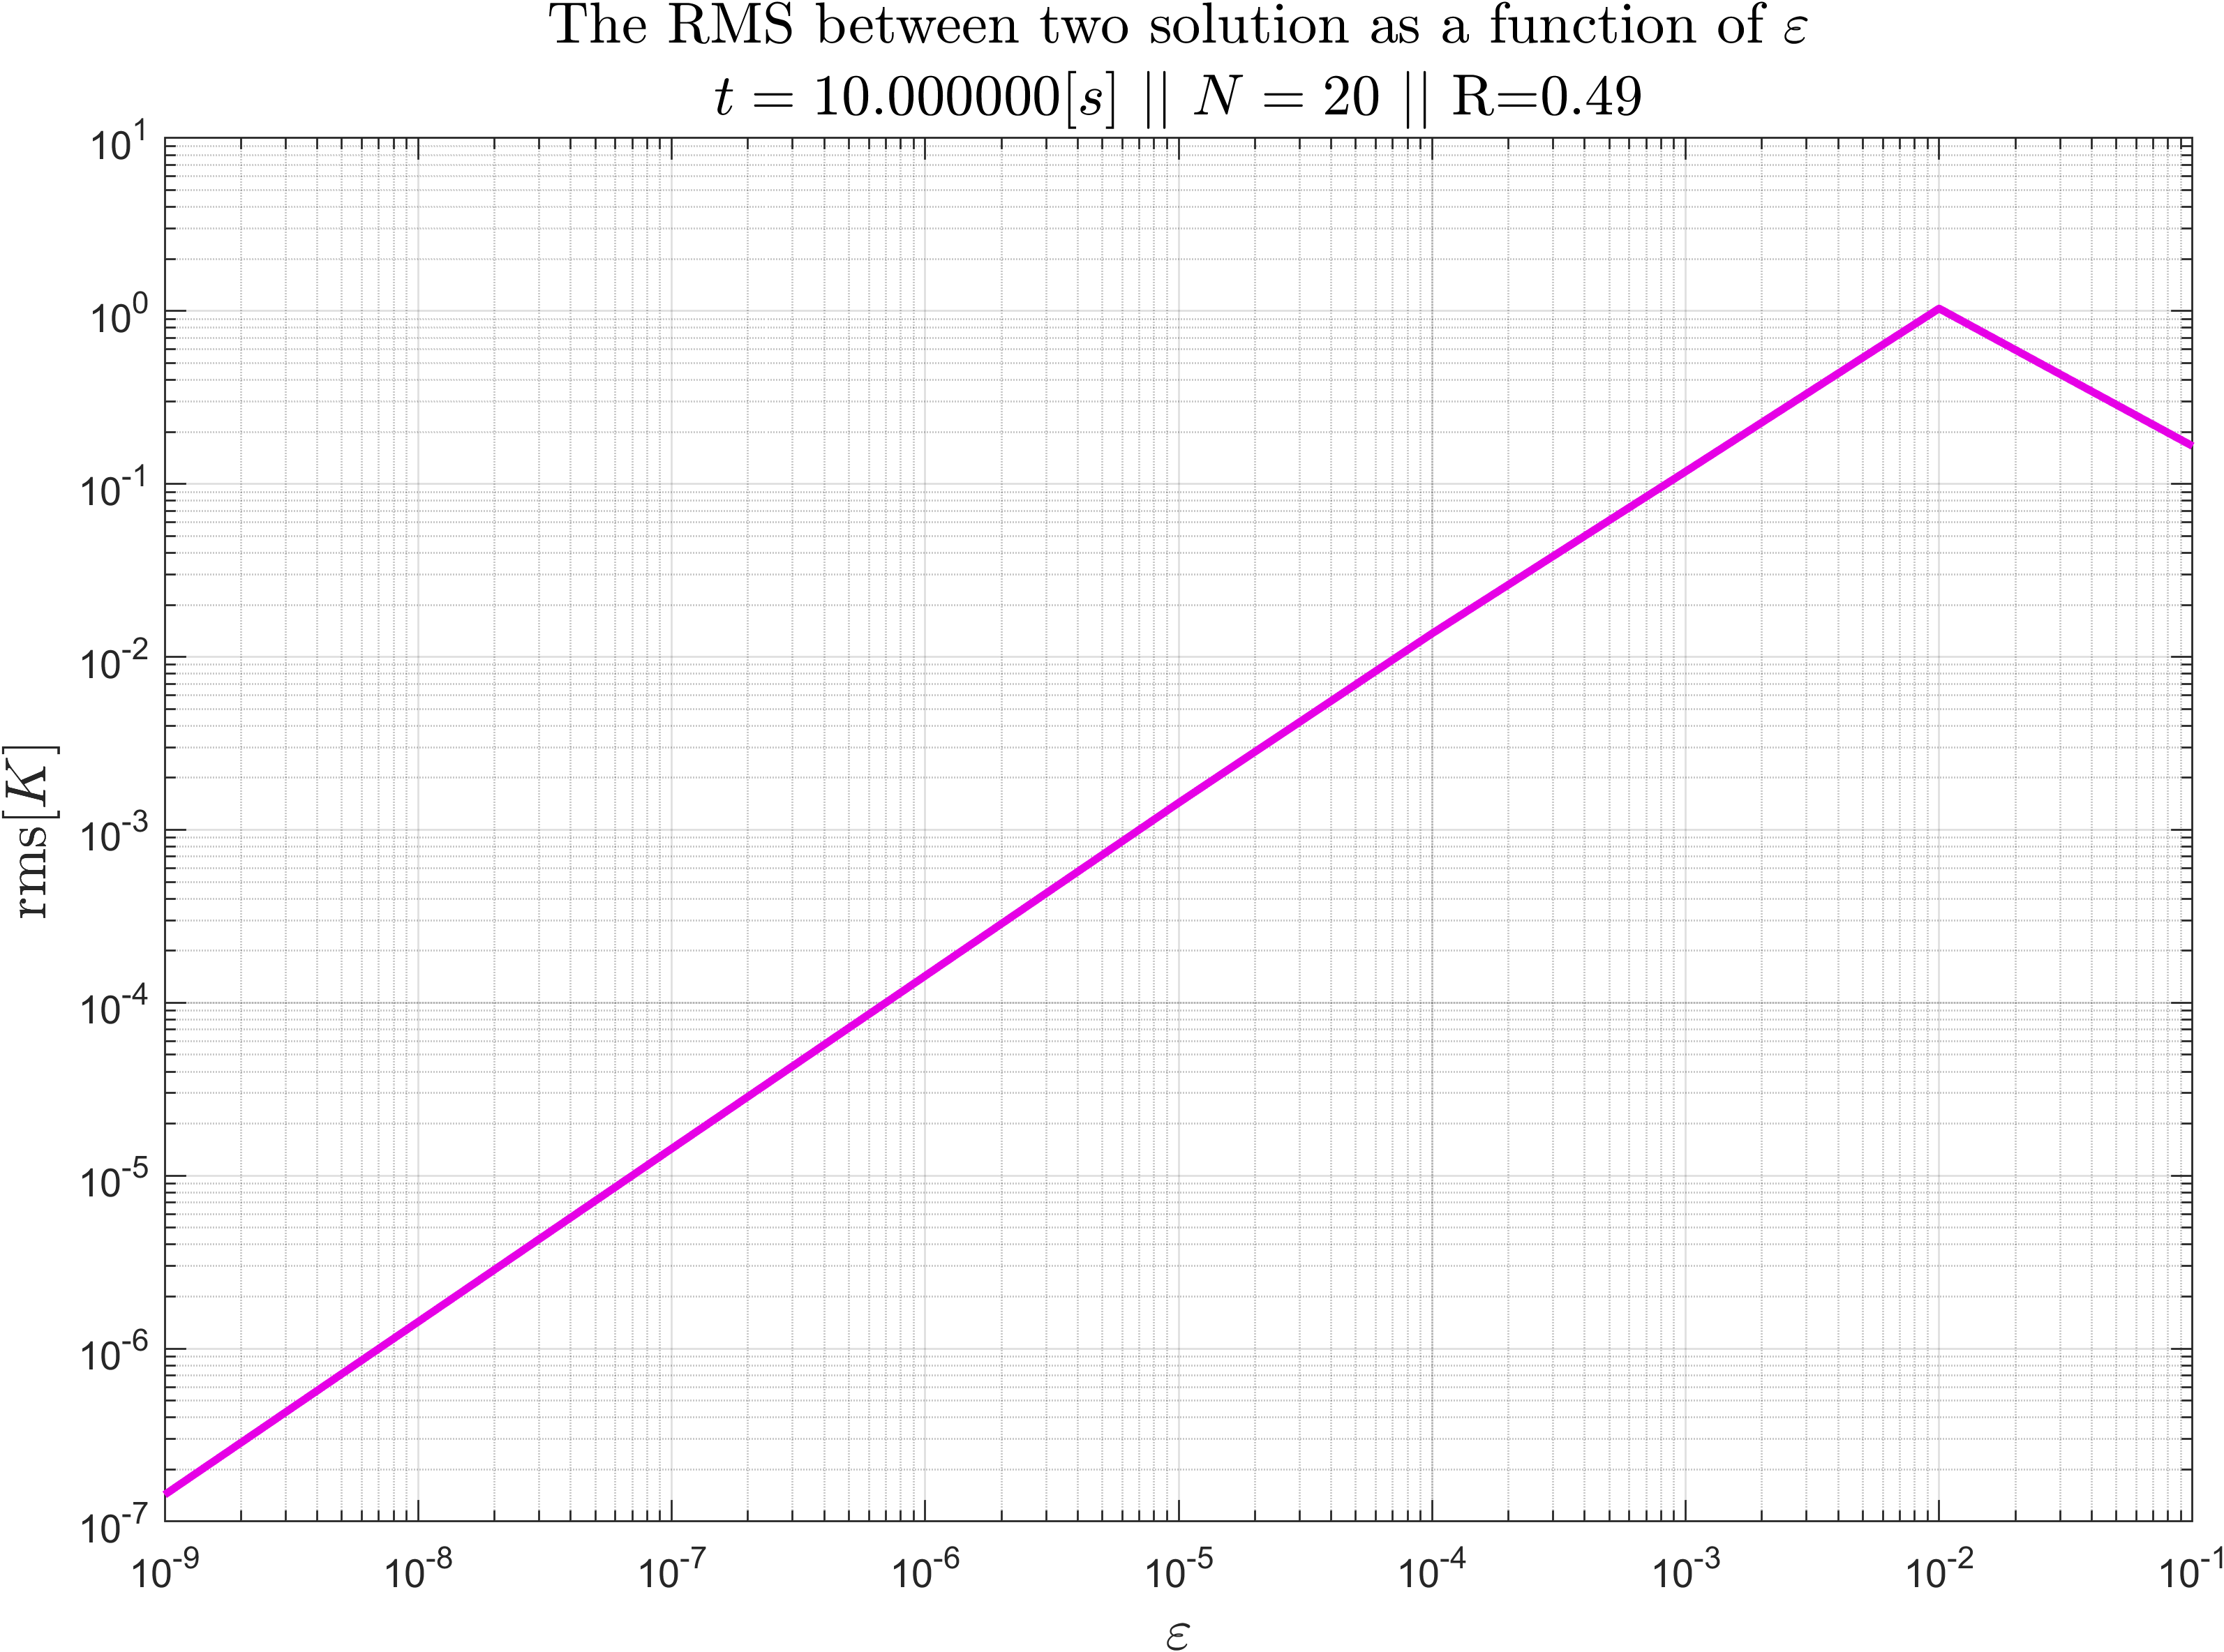
\includegraphics[width=\textwidth]{images/Influenc of epsilon - error.png}
        \caption{RMS as a function of epsilon}
        \label{fig: RMS vs epsilon}
    \end{subfigure}
    \caption{FD - Influence of the convergence criteria $\varepsilon$}
    \label{fig: Influence of epsilon}
\end{figure}
From Fig.\ref{fig: Influence of epsilon} we can conclude that for a convergence criteria smaller than $1e^{-5}$, the solution stays the same. We can determine that $\varepsilon=1e^{-5}$ is a good choice.

\subsection{Influence of The Numerical Parameter R}
\begin{figure}[H]
    \centering
    \begin{subfigure}[c]{0.49\textwidth}
        \centering
        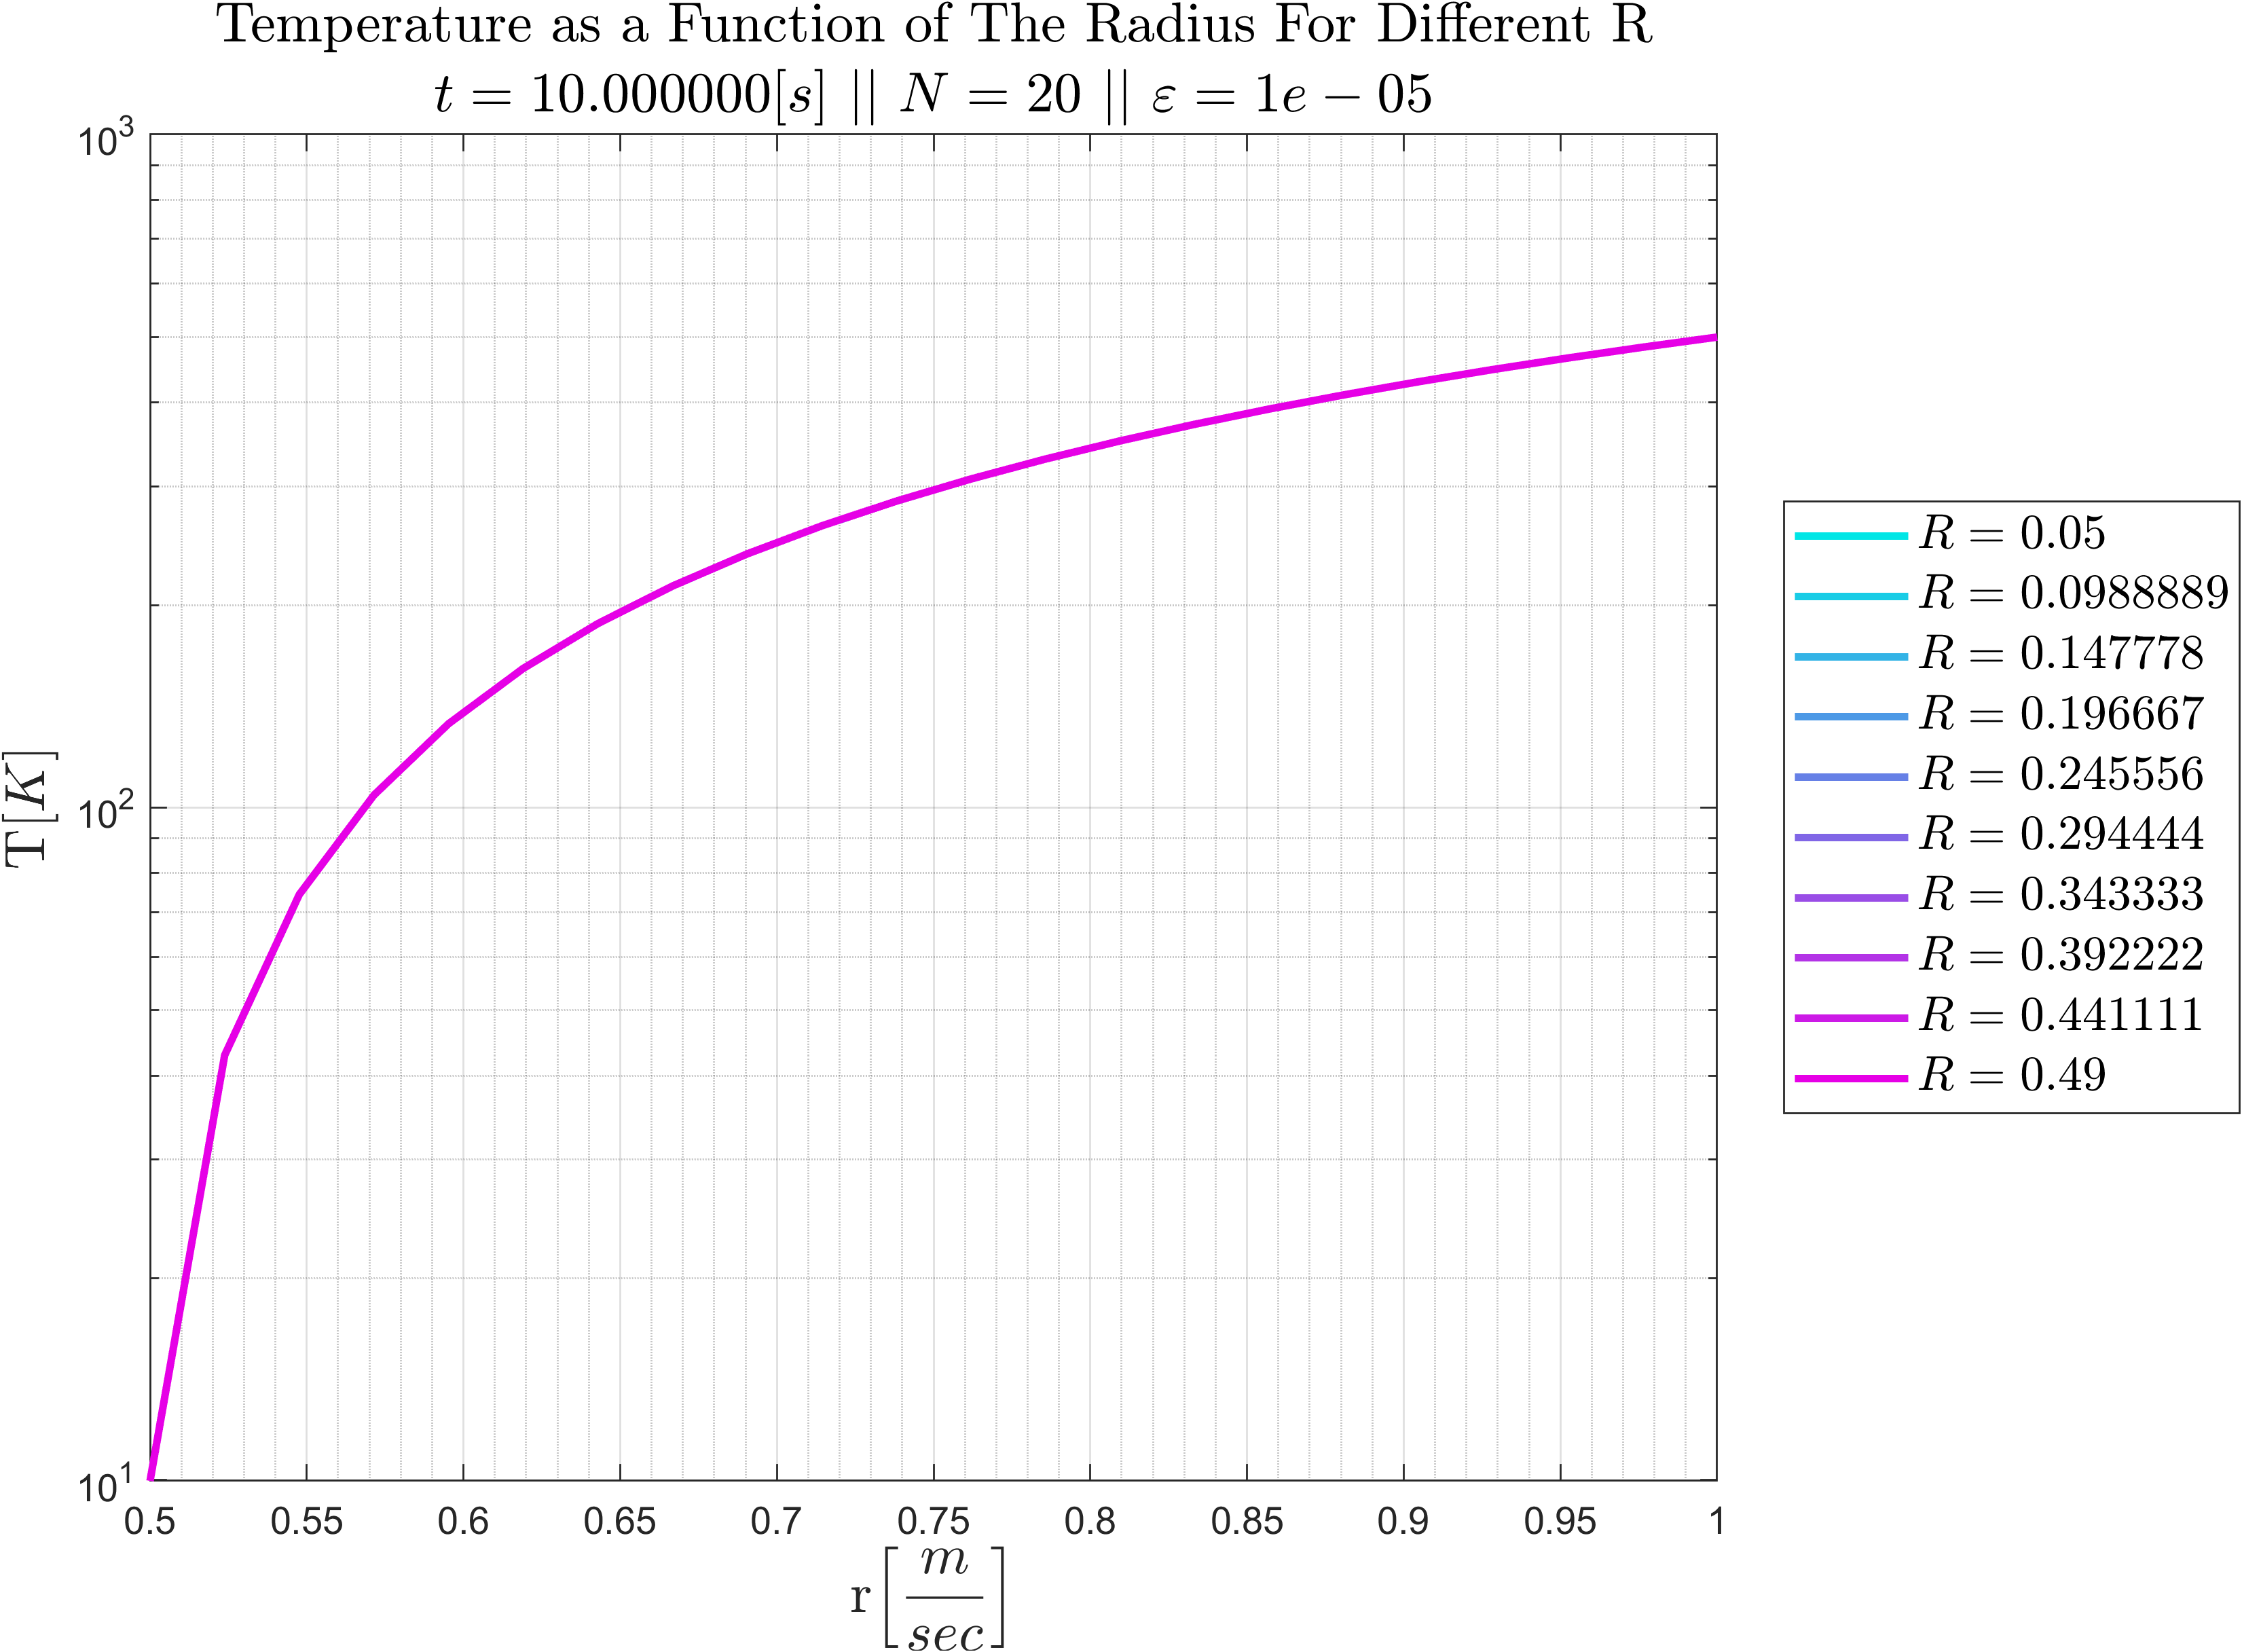
\includegraphics[width=\textwidth]{images/Influenc of R.png}
        \caption{Temperature as a Function of r for different R}
        \label{fig: T vs r for diff R}
    \end{subfigure}
    \hfill
    \begin{subfigure}[c]{0.49\textwidth}
        \centering
        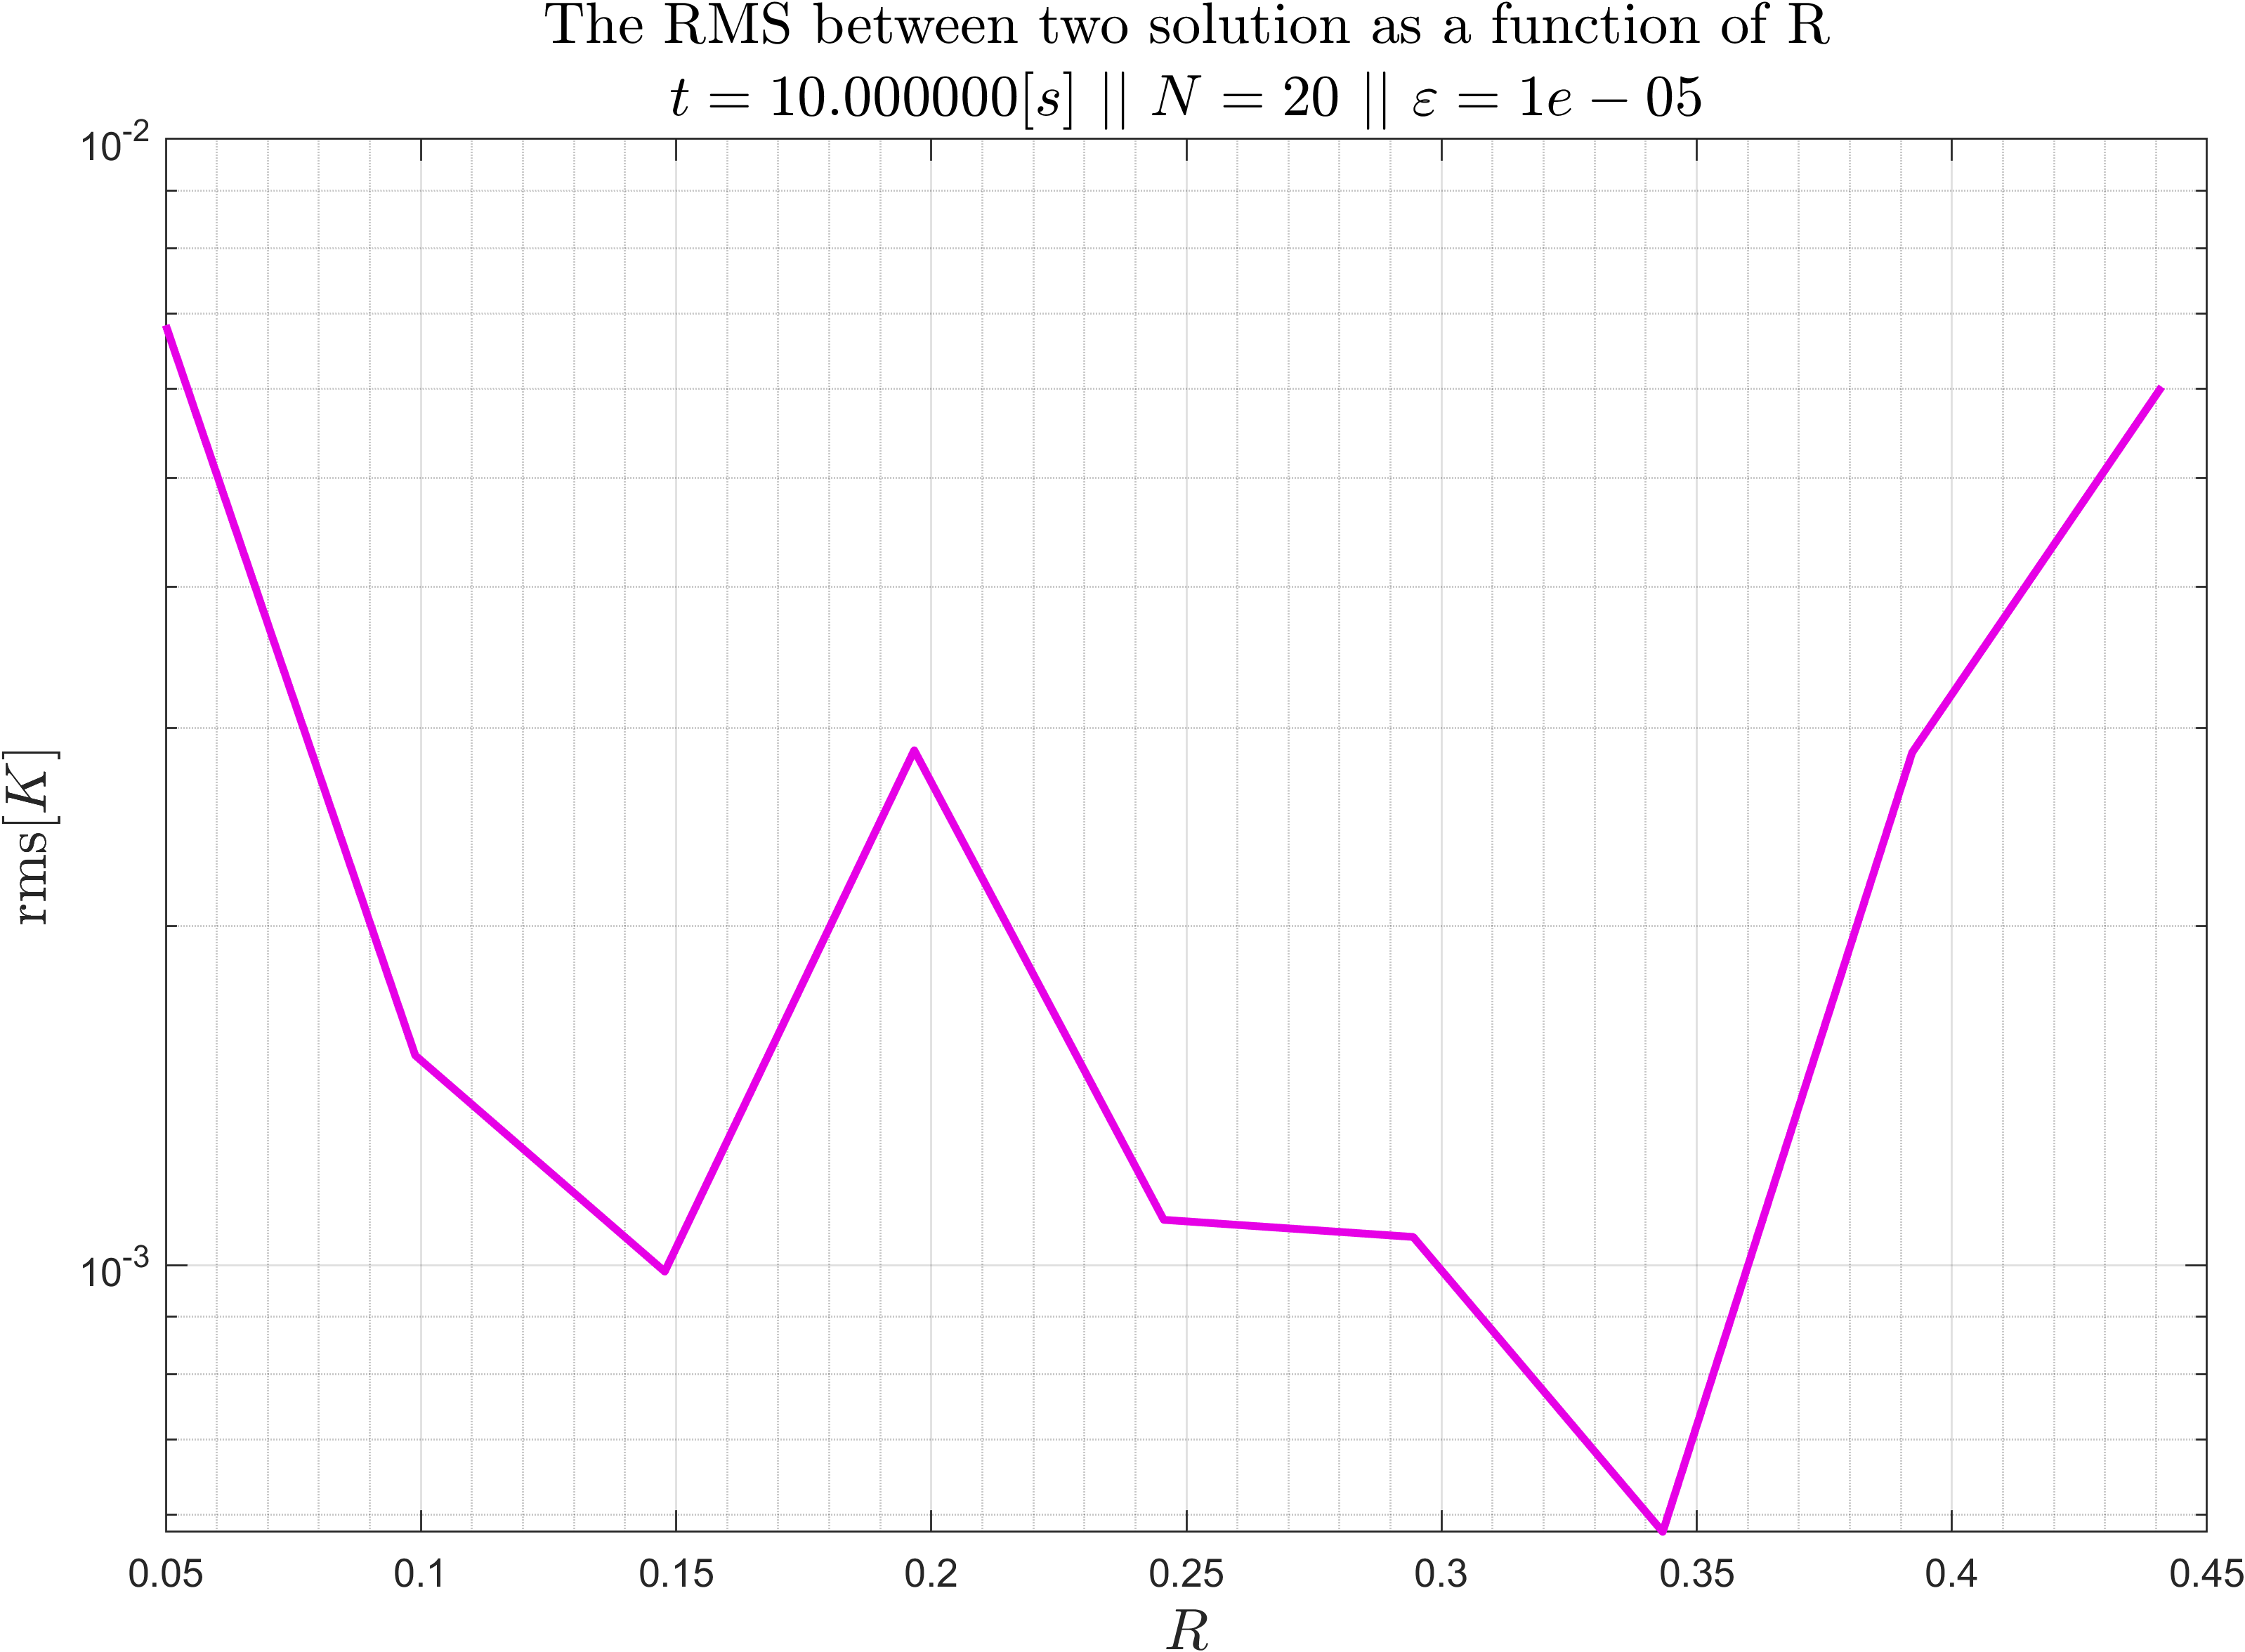
\includegraphics[width=\textwidth]{images/Influenc of R - error.png}
        \caption{RMS as a function of R}
        \label{fig: RMS vs R}
    \end{subfigure}
    \caption{FD - Influence of the convergence criteria R}
    \label{fig: Influence of R}
\end{figure}
From Fig.\ref{fig: Influence of R} we can conclude that the value of the numerical parameter R has close to no effect on the error of the solution. Therefor the chosen \emph{R} is 0.45.

\newpage
\section{Results and Discussion}
\label{sec: results and discussion}
\subsection{Temperature Distribution}
Using the parameters chosen above, the temperature distribution is therefor:
\begin{figure}[H]
    \centering
    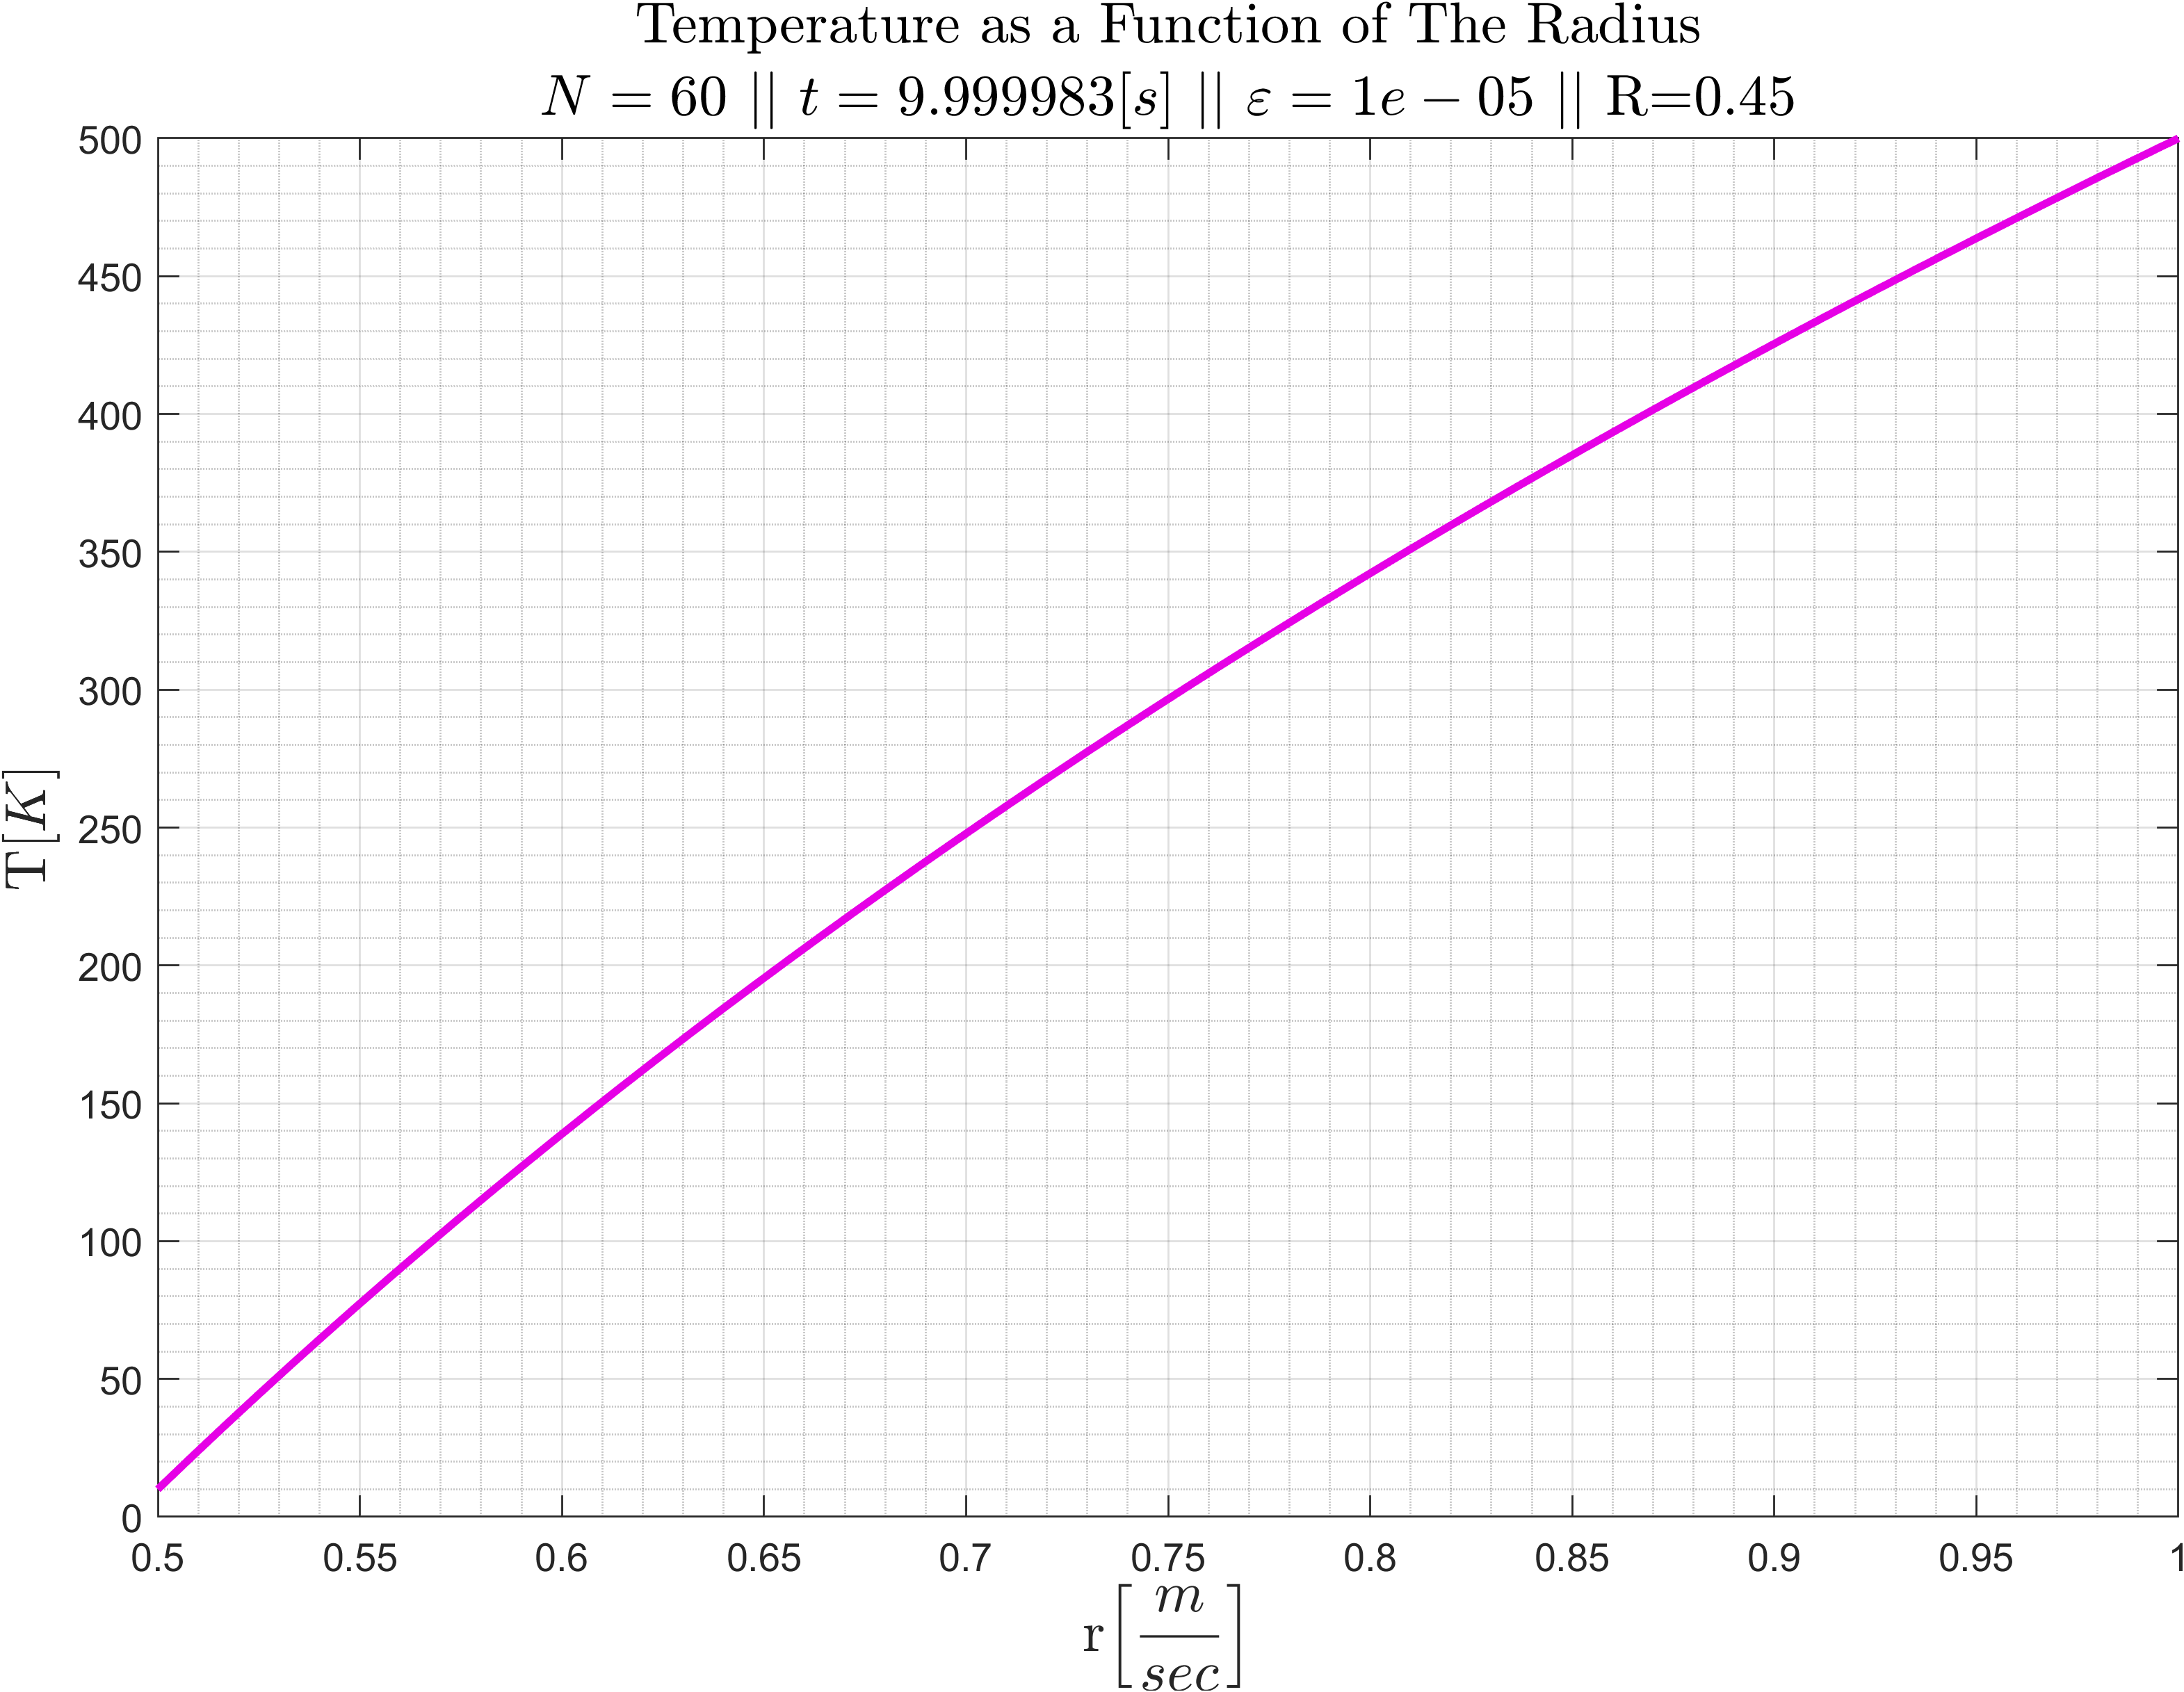
\includegraphics[width=0.7\textwidth]{images/T over r.png}
    \caption{Temperature as a Function of r}
    \label{fig: T vs r}
\end{figure}
We can also plot the temperature distribution over time for all the radiuses:
\begin{figure}[H]
    \centering
    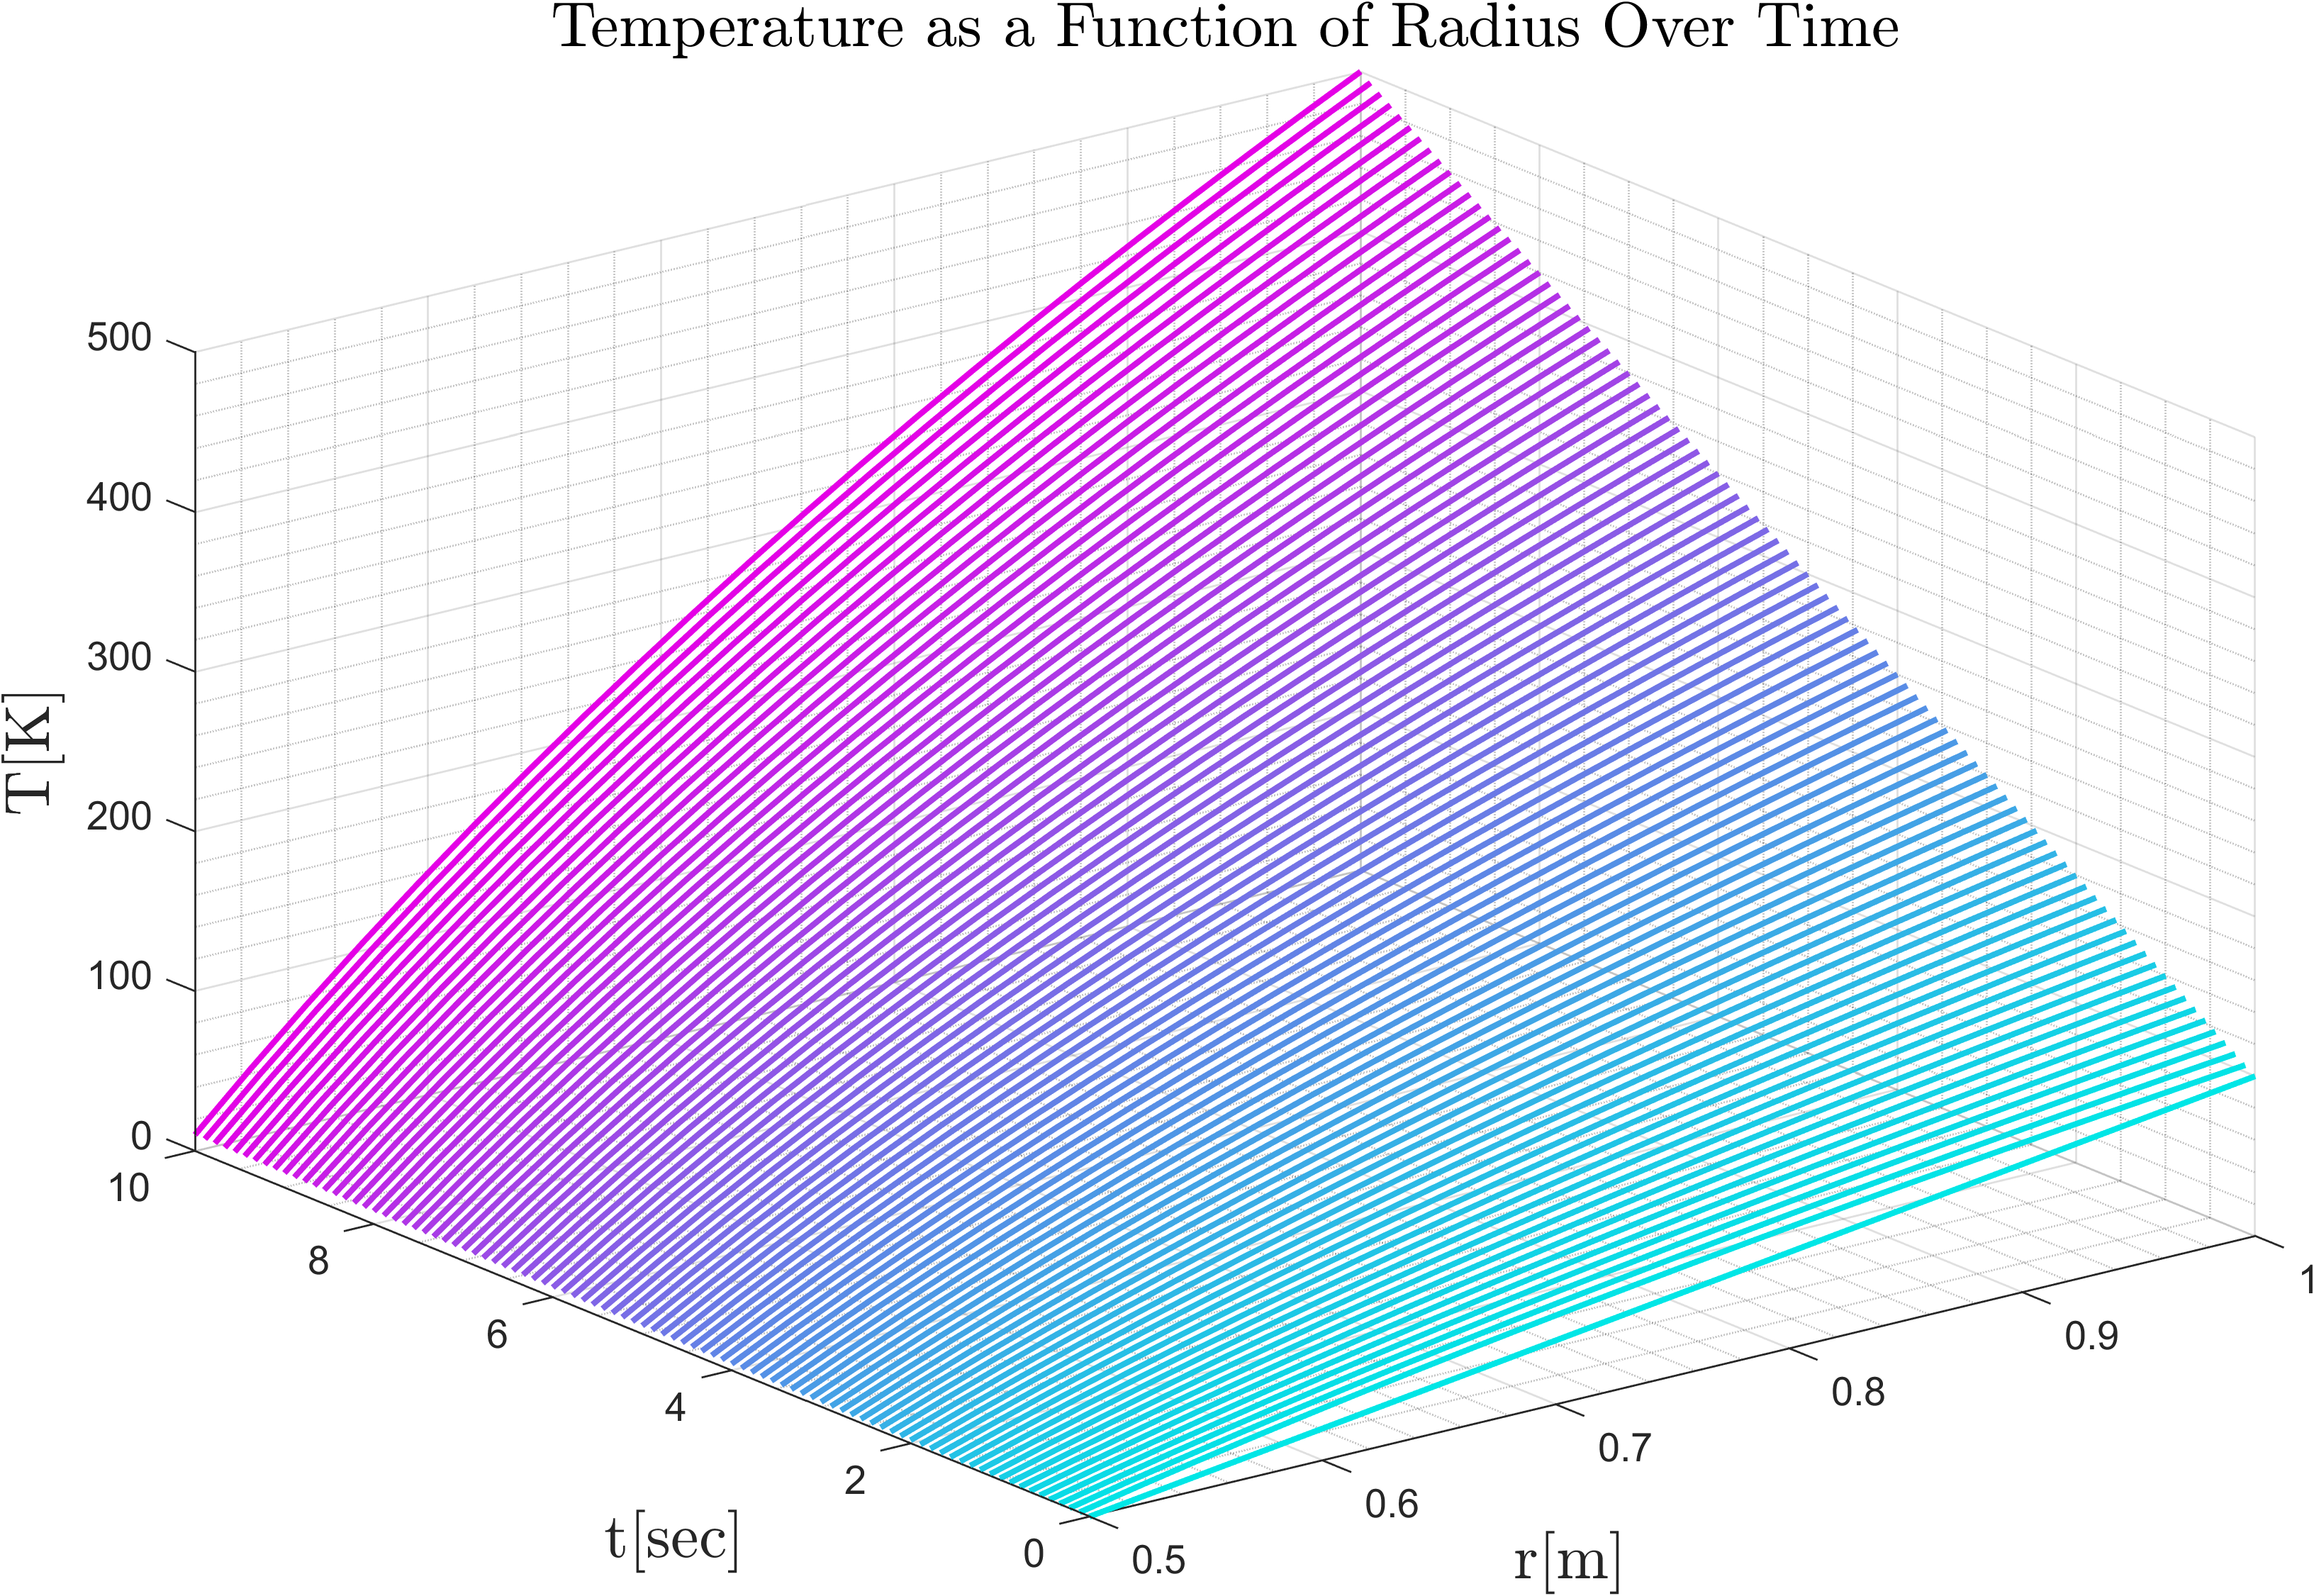
\includegraphics[width=0.7\textwidth]{images/T vs r vs t.png}
    \caption{Temperature as a Function of r over time}
    \label{fig: T vs r vs t}
\end{figure}

\newpage
\subsection{Strain Calculation}
When using the chosen parameters, the calculated strain is:
\begin{equation}
    I_{N=20}=1224.8
\end{equation}
However, when using and $N=40$ $N=60$, the strain is:
\begin{equation}
    \begin{matrix}
        I_{N=40}=1234.0 && I_{N=60}=1237.0
    \end{matrix}
\end{equation}
We observed that while $N = 20$ is adequate for convergence of the temperature, a higher number of elements is necessary to accurately calculate the strain. This is due to the order of the integration being $\emph{O}\left(h\right)$. 

\section{Summary and Conclusion}
In this assignment, a comprehensive analysis of the numerical parameters needed to solve the one-dimensional heat equation was conducted. The chosen parameters were used in the results section (Sec.\ref{sec: results and discussion}). The following conclusions came to light:
\begin{itemize}
    \item 20 elements is a sufficient number of elements for convergence of the temperature distribution, however the strain value is not yet converged at such values.
    \item The RMS of the error decreases exponentially with the decrease of the convergence criteria.
    \item The numerical parameter \emph{R} has near to no effect on the convergence of the temperature distribution.
\end{itemize}

\newpage
\appendix
\section{Listing of The Computer Program}
\subsection{Parameters}
\begin{lstinputlisting}[captionpos=b,stringstyle=\color{magenta},frame=single, numbers=left, style=MatLab-editor, basicstyle=\mlttfamily\small, caption={Parameters file},mlshowsectionrules=true]{./matlab/parameters.m}
\end{lstinputlisting}

\subsection{Main Code}
\begin{lstinputlisting}[captionpos=b,stringstyle=\color{magenta},frame=single, numbers=left, style=MatLab-editor, basicstyle=\mlttfamily\small, caption={The main file},mlshowsectionrules=true]{./matlab/NM_hw2_CA.m}
\end{lstinputlisting}

\end{document}